\section{Pregunta 1 (0.2 puntos)}

\begin{figure}[H]
    \centering
    \begin{subfigure}[b]{0.9\textwidth}
        \centering
        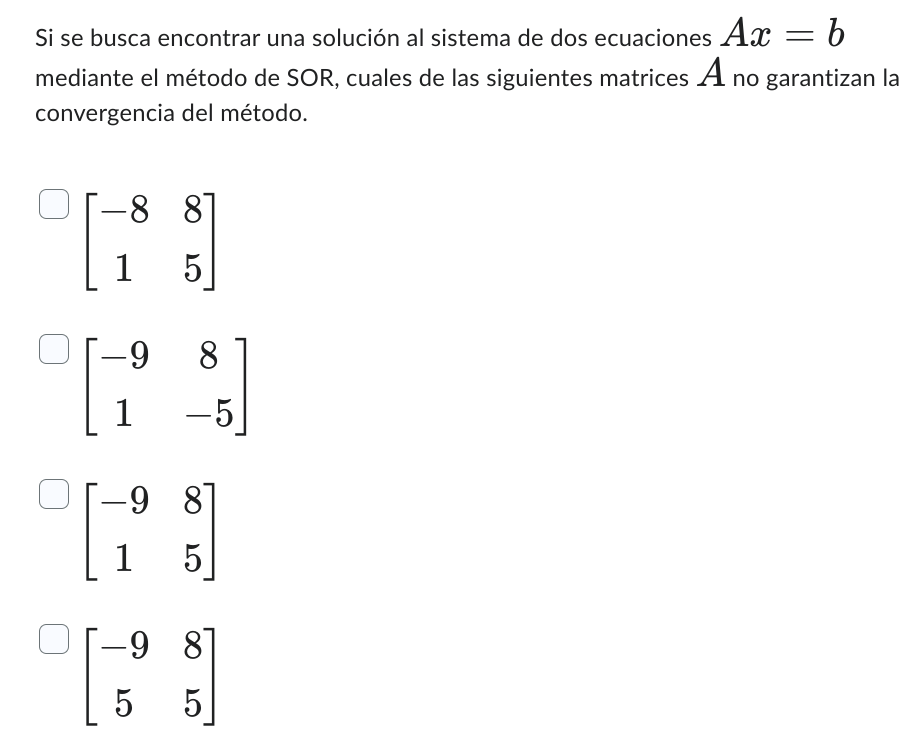
\includegraphics[width=0.9\textwidth]{Figures/0. General/1.png}
        \caption{Pregunta 1}
        \label{fig: pregunta 1}
    \end{subfigure}
\end{figure}

El método de SOR es una técnica iterativa para resolver sistemas de ecuaciones lineales, y una condición necesaria para la convergencia del método de SOR es que la matriz \( A \) sea simétrica y definida positiva (en el caso de matrices reales), o al menos que la matriz sea diagonalmente dominante.

Una matriz es diagonalmente dominante si para cada fila, el valor absoluto del elemento de la diagonal es mayor que la suma de los valores absolutos de los otros elementos de esa fila. También hay una condición más débil de convergencia que es la semidefinida positividad para matrices simétricas.

Veamos las matrices una por una:

1. \(\begin{bmatrix}-8 & 8\\ 1 & 5\end{bmatrix}\)
Esta matriz no es diagonalmente dominante ya que \( |-8| < |8| \) y \( |5| \) no es mayor que \( |1| \) (no cumple con la condición para ninguna fila). Además, no es simétrica.

2. \(\begin{bmatrix}-9 & 8\\ 1 & -5\end{bmatrix}\)
Esta matriz tampoco es diagonalmente dominante porque \( |-9| < |8| \) y \( |-5| < |1| \). Además, tampoco es simétrica.

3. \(\begin{bmatrix}-9 & 8\\ 1 & 5\end{bmatrix}\)
Esta matriz no es diagonalmente dominante porque \( |-9| < |8| \), aunque \( |5| > |1| \). No es simétrica tampoco.

4. \(\begin{bmatrix}-9 & 8\\ 5 & 5\end{bmatrix}\)
Esta matriz no es diagonalmente dominante ya que \( |-9| < |8| \) y \( |5| < |5| \) (las sumas son ig

\section{Pregunta 2 (0.2 puntos)}

\begin{figure}[H]
    \centering
    \begin{subfigure}[b]{0.9\textwidth}
        \centering
        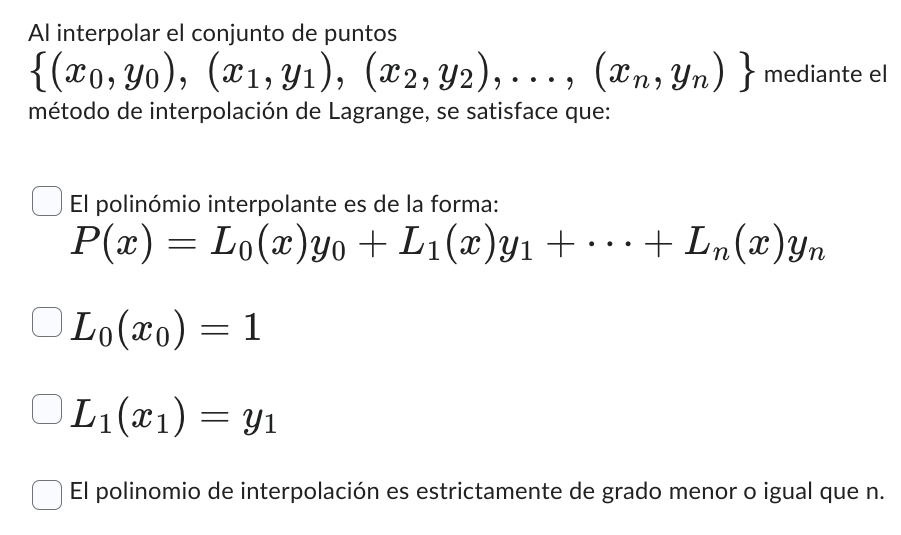
\includegraphics[width=0.9\textwidth]{Figures/0. General/2.png}
        \caption{Pregunta 2}
        \label{fig: pregunta 2}
    \end{subfigure}
\end{figure}

El método de interpolación de Lagrange es un proceso matemático utilizado para encontrar un polinomio que pase exactamente por un conjunto dado de puntos. Este método utiliza polinomios base \(L_i(x)\) que son construidos de manera que \(L_i(x_j) = \delta_{ij}\), donde \(\delta_{ij}\) es la delta de Kronecker, que vale 1 si \(i = j\) y 0 si \(i \neq j\).

1. El polinomio interpolante es de la forma:
\[ P(x) = L_0(x)y_0 + L_1(x)y_1 + \ldots + L_n(x)y_n \]
Esta afirmación es verdadera. La forma general del polinomio de interpolación de Lagrange es precisamente una combinación lineal de los polinomios base \(L_i(x)\) multiplicados por los respectivos valores de \(y\).

2. \( L_0(x_0) = 1 \)
Esta afirmación es verdadera. Por definición, el polinomio base \(L_0(x)\) está diseñado de tal manera que \(L_0(x_0) = 1\) y \(L_0(x_j) = 0\) para todo \(j \neq 0\).

3. \( L_1(x_1) = y_1 \)
Esta afirmación es falsa. \(L_1(x_1)\) debería ser igual a 1, no a \(y_1\). La función de Lagrange \(L_i(x)\) en \(x = x_i\) siempre es 1 para su propio índice y 0 para todos los demás.

4. El polinomio de interpolación es estrictamente de grado menor o igual que \(n\).
Esta afirmación es verdadera. El polinomio de interpolación de Lagrange construido a partir de \(n+1\) puntos (\(n\) es el índice máximo, por lo que hay \(n+1\) puntos desde \(x_0\) hasta \(x_n\)) es siempre de grado \(n\) o menor o igual a \(n\).

\section{Pregunta 3 (0.2 puntos)}
\begin{figure}[H]
    \centering
    \begin{subfigure}[b]{0.9\textwidth}
        \centering
        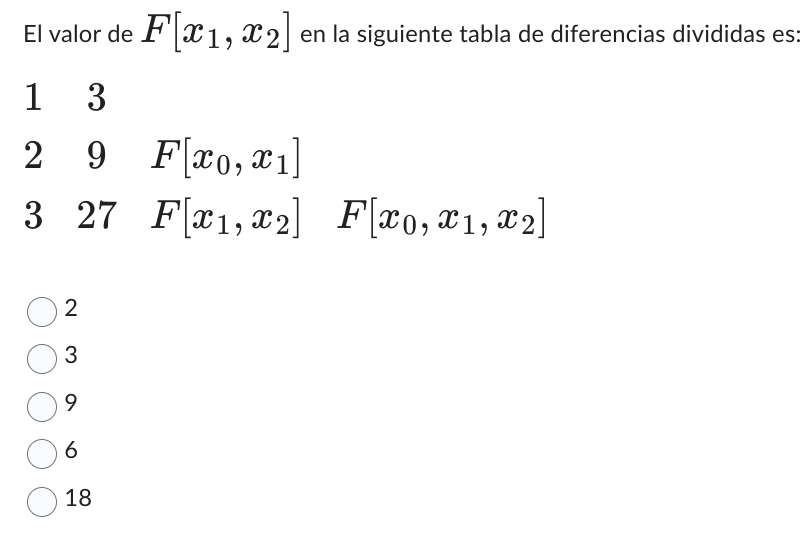
\includegraphics[width=0.9\textwidth]{Figures/0. General/3.png}
        \caption{Pregunta 3}
        \label{fig: pregunta 3}
    \end{subfigure}
\end{figure}

Para calcular la diferencia dividida \( F[x_1, x_2] \), usamos la fórmula de las diferencias divididas de Newton, que para dos puntos es:

\[ F[x_1, x_2] = \frac{F(x_2) - F(x_1)}{x_2 - x_1} \]

Mirando la tabla proporcionada, tenemos los siguientes valores:

- \( F(x_1) = 9 \)
- \( F(x_2) = 27 \)
- \( x_1 = 2 \)
- \( x_2 = 3 \)

Sustituyendo estos valores en la fórmula obtenemos:

\[ F[x_1, x_2] = \frac{27 - 9}{3 - 2} = \frac{18}{1} = 18 \]

Por lo tanto, la respuesta correcta es \( 18 \).


\section{Pregunta 4 (0.2 puntos)}

\begin{figure}[H]
    \centering
    \begin{subfigure}[b]{0.9\textwidth}
        \centering
        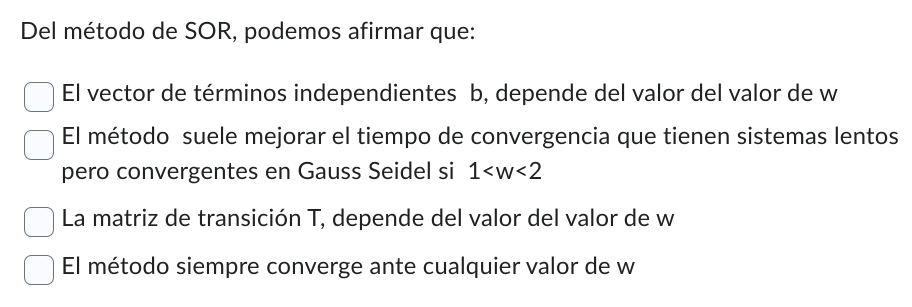
\includegraphics[width=0.9\textwidth]{Figures/0. General/4.png}
        \caption{Pregunta 4}
        \label{fig: pregunta 4}
    \end{subfigure}
\end{figure}


\begin{itemize}
    \item El vector de términos independientes \( b \), depende del valor del valor de \( w \):
          \subitem Esta afirmación es falsa. El vector \( b \) es parte del sistema de ecuaciones \( Ax = b \) y no depende del factor de relajación \( w \). El factor de relajación se usa para acelerar la convergencia de la solución.

    \item El método suele mejorar el tiempo de convergencia que tienen sistemas lentos pero convergentes en Gauss Seidel si \( 1 < w < 2 \):
          \subitem \textbf{Esta afirmación es verdadera}. El método de SOR puede mejorar la tasa de convergencia del método de Gauss-Seidel si se elige un valor apropiado para \( w \) en el intervalo \( (1, 2) \).

    \item La matriz de transición \( T \), depende del valor del valor de \( w \):
          \subitem \textbf{Esta afirmación es verdadera}. La matriz de transición en el método SOR, que define cómo se pasa de una iteración a la siguiente, efectivamente depende del valor del factor de relajación \( w \).

    \item El método siempre converge ante cualquier valor de \( w \):
          \subitem Esta afirmación es falsa. El método de SOR no garantiza la convergencia para cualquier valor de \( w \). El rango efectivo para \( w \) donde se puede esperar convergencia es generalmente entre \( 0 \) y \( 2 \), pero la convergencia está garantizada bajo ciertas condiciones y para ciertas matrices si \( w \) se elige en el intervalo \( (1, 2) \).
\end{itemize}

\section{Pregunta 5 (0.2 puntos)}

\begin{figure}[H]
    \centering
    \begin{subfigure}[b]{0.9\textwidth}
        \centering
        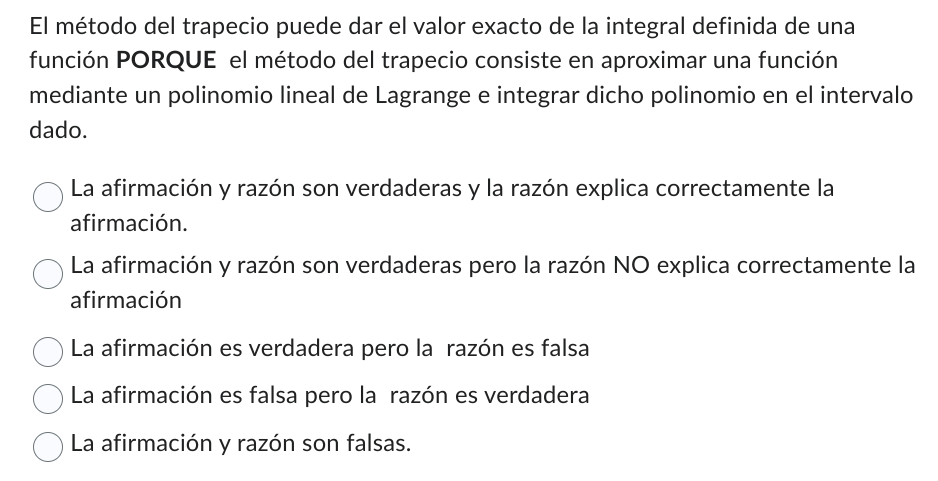
\includegraphics[width=0.9\textwidth]{Figures/0. General/5.png}
        \caption{Pregunta 5}
        \label{fig: pregunta 5}
    \end{subfigure}
\end{figure}

La afirmación dice: "El método del trapecio puede dar el valor exacto de la integral definida de una función PORQUE el método del trapecio consiste en aproximar una función mediante un polinomio lineal de Lagrange e integrar dicho polinomio en el intervalo dado".

La afirmación en la primera parte es cierta bajo ciertas circunstancias. El método del trapecio puede dar el valor exacto de la integral definida de una función cuando la función es lineal o cuando se usa un número infinito de trapecios (lo que en el límite se convierte en la integral definida).

La razón dada, sin embargo, es ligeramente engañosa. Si bien es cierto que el método del trapecio aproxima el área bajo la curva usando un polinomio lineal, que en el caso más simple podría ser visto como el polinomio de Lagrange de primer grado (lineal) entre dos puntos, no se suele explicar en términos del polinomio de Lagrange. El método del trapecio es un caso particular de la regla de Newton-Cotes para n=1. Aunque el resultado final de ambos métodos puede parecer similar (una línea recta que aproxima la función entre dos puntos), no se define específicamente como una aproximación por polinomios de Lagrange en la mayoría de los textos.

Dicho esto, la mejor opción sería:

La afirmación y razón son verdaderas pero la razón NO explica correctamente la afirmación.

\section{Pregunta 6, Norman se fue de sábatico cariño (4 puntos)}

En capítulos anteriores vimos que el Duende verde se había postulado para ser alcalde de Metrallo, y efectivamente salió elegido. Esto se debió principalmente, gracias  a su alianza con Kingpin, el cual buscaba ser elegido gobernador e implementar la propuesta del Duende de bombardear las comunas, pero con la idea de bombardear todo el departamento. Ante la problemática inminente de un departamento bombardeado, Spiderman debe encontrar las coordenadas de los lugares donde se realizaran los bombardeos (c corresponde al último dígito de su cédula)

\subsection{1 pt}

Sabiendo que algunos de estos bombardeos ya fueron ejecutados en la piedra del peñol ($x=5$), en un puente por allá en santa fe de Antioquia ($x=4$),  en una urna de votación en la estrella ($x=3$) y en un restaurante en Bello  ($x=1$). Ayude a Spiderman a calcular las $y_i$ correspondientes a cada ubicación, sabiendo que estas corresponden a la cantidad de iteraciones que tarda el método de Jacobi para resolver el siguiente sistema de ecuaciones:

\[
    \begin{bmatrix}
        11 - x & 5     & 6 \\
        -2     & 4 + c & 1 \\
        -1     & -1    & 4
    \end{bmatrix}
    \begin{bmatrix}
        z_1 \\
        z_2 \\
        z_3
    \end{bmatrix}
    =
    \begin{bmatrix}
        15 \\
        15 \\
        20
    \end{bmatrix}
    \quad
    x_0 =
    \begin{bmatrix}
        1 \\
        1 \\
        1
    \end{bmatrix}
\]

$tol = 2$ cifras significativas


\begin{itemize}
    \item La solución para $x=5$ es $[-2.94521073,  1.14308638,  4.53881968]$ y el número de iteraciones es 34
    \item La solución para $x=4$ es $[-2.69108719,  1.26848927,  4.64375115]$ y el número de iteraciones es 22
    \item La solución para $x=3$ es $[-2.47890361,  1.35605757,  4.72274498]$ y el número de iteraciones es 18
    \item La solución para $x=1$ es $[-2.13507286,  1.49511276,  4.84595027]$ y el número de iteraciones es 14
\end{itemize}

En síntesis la respuesta es 34, la cantidad de iteraciones que tarda el método de Jacobi para resolver
el sistema de ecuaciones anterior es 34.

\subsection{1 pt}

Peter cree que el siguiente ataque será cerca de Caucacia, por lo que pone el valor de ($x=11$) "bien en la puta mierda", en el método y nota que algo extraño sucede en el método, mientras que en las otras ciudades si había. Verifique que pasó en el método y dé una explicación a Peter sobre las razones que llevan a este suceso, para que no vaya hasta por allá a que lo levanten a plomo.

\begin{itemize}
    \item  Al final no se puede porque la iteración 100 se divide por 100, por lo que se daña
\end{itemize}

\subsection{1 pt}

Al final a Spiderman es más gráfico y requiere de un polinomio que interpole los datos para él saber donde caer ante un bombardeo. Entregue una gráfica del polinomio interpolante de Vandermonde, e indique la coordenada $y$ correspondiente a un ataque en Barbosa ($x=1.5$) .

\begin{itemize}
    \item La solución para $x=1.5$ es $[-2.24096294,  1.43777514,  4.81437577]$ y el número de iteraciones es 15
\end{itemize}

\subsection{1 pt}

Al final a Spiderman lo terminan matando las Bacrim y ahora debemos ayudar a Miles Morales a encontrar el cuerpo de Peter. Para esto Miles cuenta con los siguientes polinomios de Spline cuadrático de los siguientes datos \( x = [7\ 8\ 9] \). Ayude a Miles a verificar el cumplimiento de las condiciones del Spline si solo se conoce \( y_0 = -1 \) y \( y_2 = -C \). Puede hacerlo gráficamente o analíticamente.

\[
    P_1(x) = x - 8 \quad 7 \leq x \leq 8
\]

\[
    P_2(x) = (c - 1)x^2 + (16c + 17)x - (64c + 72)  \quad 8 \leq x \leq 9
\]

